%inputsP2_DXpvd_woutputsP5_DX-3.tex

\begin{figure}[htbp]
	\centering 
	\subfloat[T2 DX: Narx identification]{
		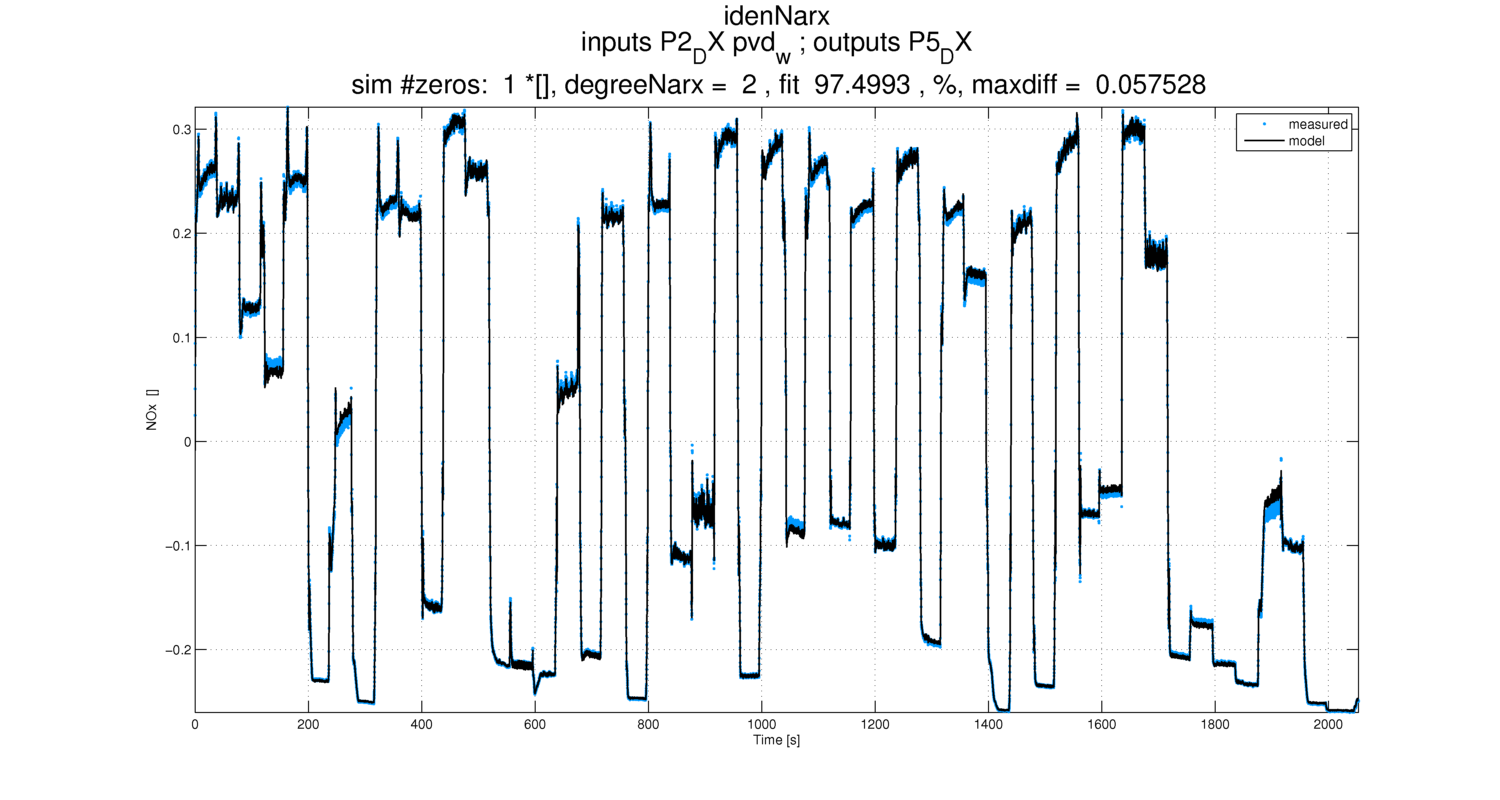
\includegraphics[width=.90\columnwidth]{Immagini/inputsP2_DXpvd_woutputsP5_DX-idenNarx-3}
		\label{fig:inputsP2_DXpvd_woutputsP5_DX-idenNarx-3}	}
	\\
	\subfloat[T2 DX: Narx prediction]{
		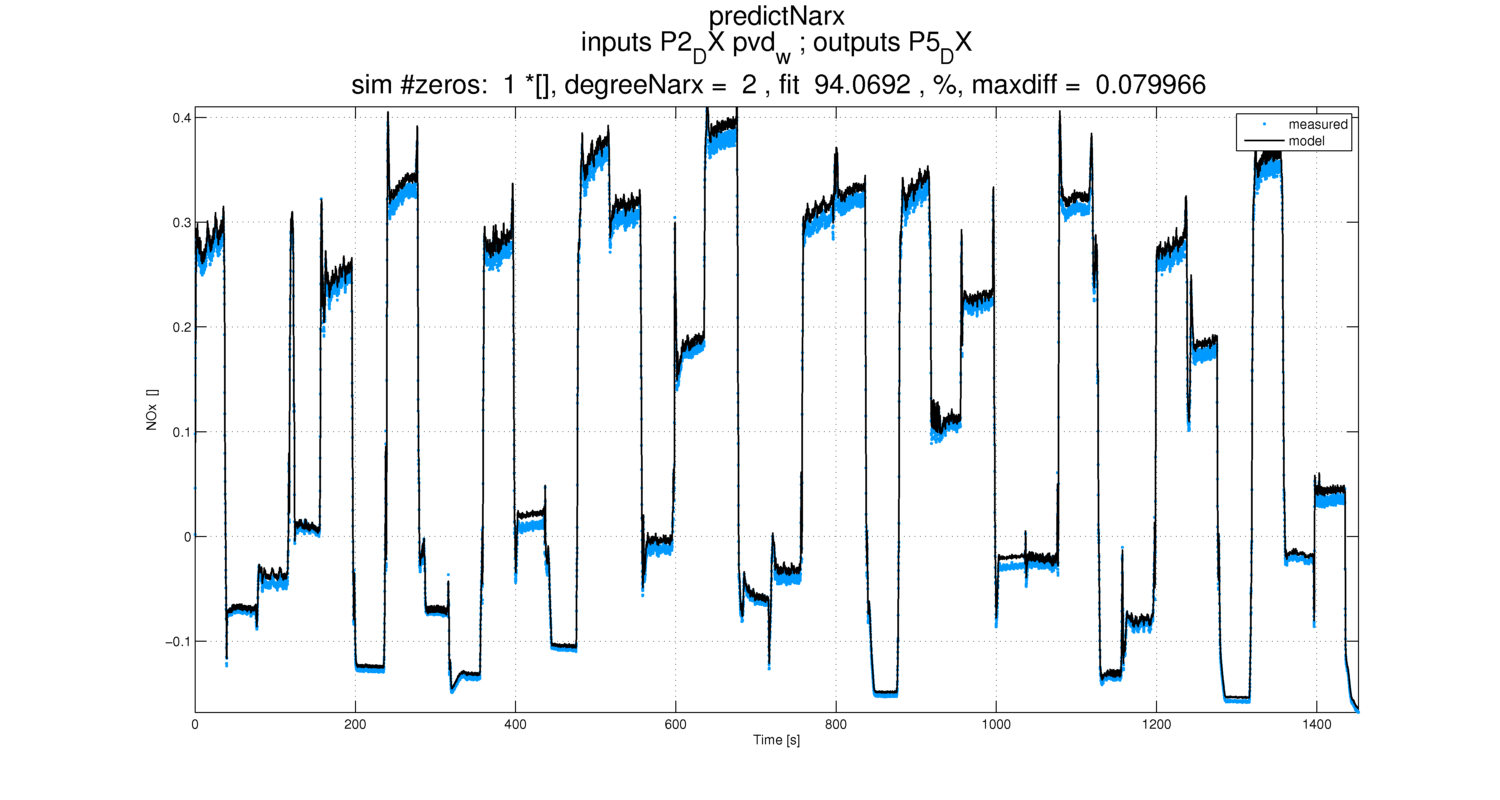
\includegraphics[width=.90\columnwidth]{Immagini/inputsP2_DXpvd_woutputsP5_DX-predictNarx-3}
		\label{fig:inputsP2_DXpvd_woutputsP5_DX-predictNarx-3}
	}
	\\
	\subfloat[T2 DX: Narx simulation]{
		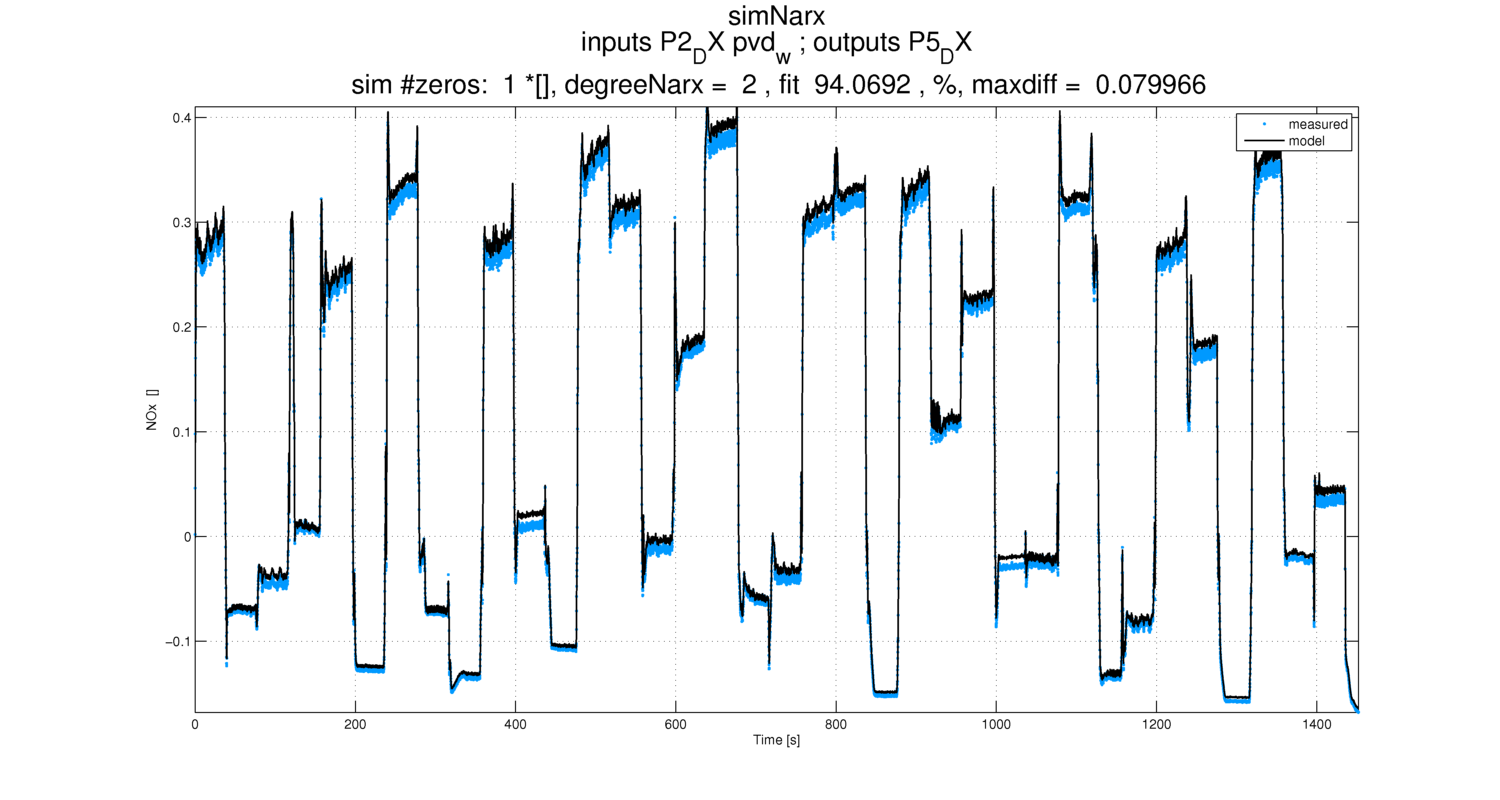
\includegraphics[width=.90\columnwidth]{Immagini/inputsP2_DXpvd_woutputsP5_DX-simNarx-3}
		\label{fig:inputsP2_DXpvd_woutputsP5_DX-simNarx-3}
	}
\phantomcaption
\end{figure}


\begin{figure}[htbp] \ContinuedFloat
	\centering 
	\subfloat[T2 DX: Transfer function identification]{
		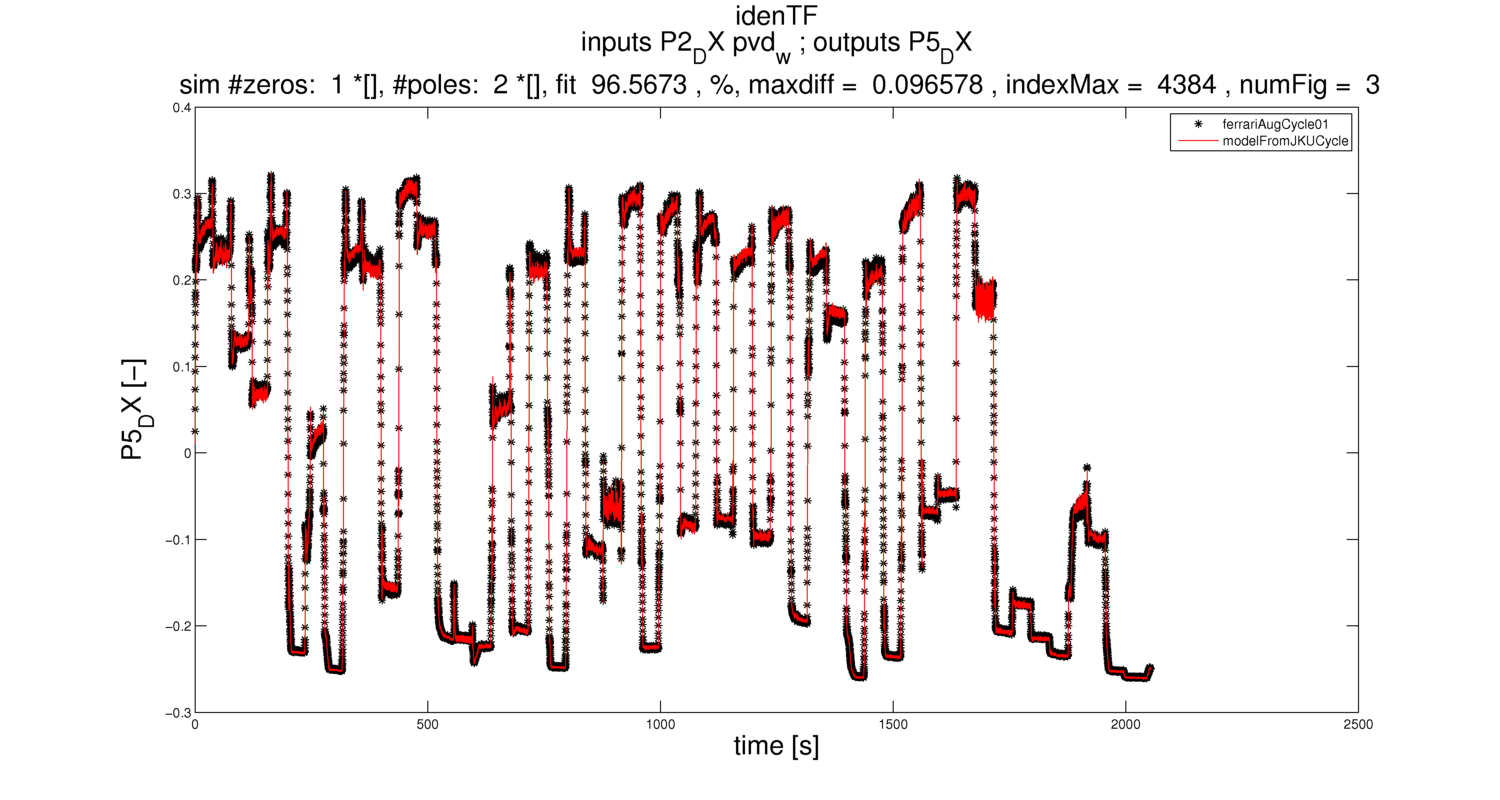
\includegraphics[width=.90\columnwidth]{Immagini/inputsP2_DXpvd_woutputsP5_DX-idenTF-3}
		\label{fig:inputsP2_DXpvd_woutputsP5_DX-idenTF-3}  }
	\\
	\subfloat[T2 DX: Transfer function simulation]{
		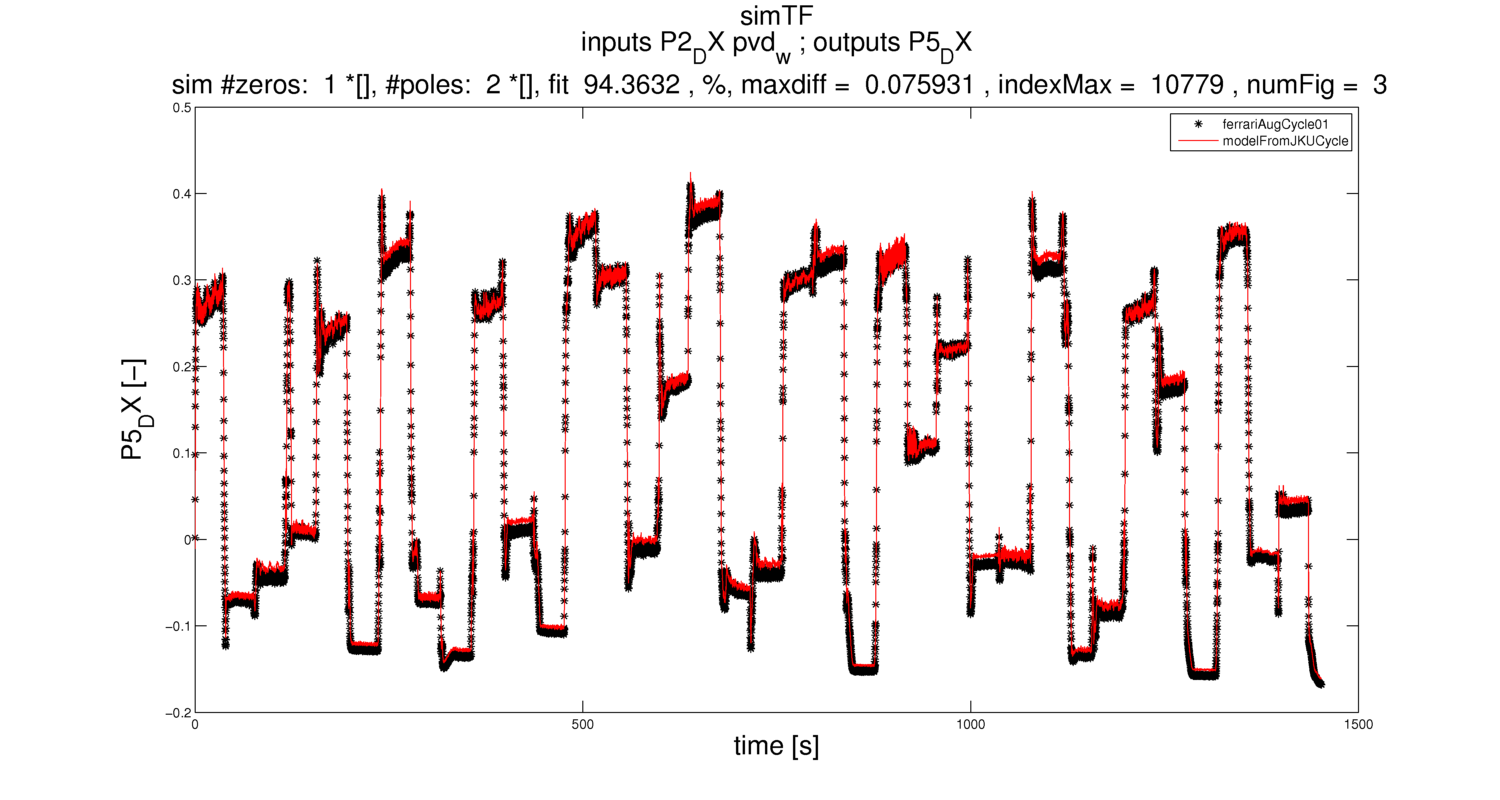
\includegraphics[width=.90\columnwidth]{Immagini/inputsP2_DXpvd_woutputsP5_DX-simTF-3}
		\label{fig:inputsP2_DXpvd_woutputsP5_DX-simTF-3}  }
	\\	
	\caption[Inputs: P2 DX, pvd w; Output: P5 DX; np: 2; nz: 1; degree: 2]{Inputs: P2 DX, pvd w; Output: P5 DX; np: 2; nz: 1; degree: 2.}
	\label{fig:inputsP2_DXpvd_woutputsP5_DX-3}
\end{figure}